\chapter{Methods and experimental setup}\label{ch:methods}
\thispagestyle{pagestyle}

\graphicspath{{../../outputs/}{images/}{../../thesis/design/figures/}}

\section{Pipeline overview}
\label{sec:pipeline-overview}
The method is a single pipeline that turns a grayscale image into an edge map and a handful of quality scores. \Cref{fig:pipeline-flow} shows the stages end to end. A test image is encoded into an FRQI quantum state, where each pixel intensity becomes a rotation angle on one shared color qubit. That state is simulated on Qiskit Aer, either exactly as a statevector or, when noise is added, as a density matrix. The simulated state is decoded back into an ordinary $N\times N$ raster. The reconstructed raster is passed through the quantum Hadamard edge detector (QHED) and compared against a classical Sobel edge map. Finally, the reconstruction and the edge maps are scored with PSNR, SSIM, edge SSIM, and state fidelity.

The key point for the experiments is that only the first box changes between runs: the FRQI \emph{preparation unitary} (naive versus v-chain synthesis) and, in the noisy runs, the noise channel attached to it. Decoding, QHED, the Sobel reference, and the metrics are held fixed, so any difference in scores can be attributed to preparation rather than to the detector or the scoring code.

\begin{figure}[htbp]
\centering
\resizebox{\textwidth}{!}{%
\begin{tikzpicture}[
  font=\small,
  box/.style={rectangle, draw, rounded corners=2pt, align=center, inner sep=5pt, minimum width=2.2cm},
  arrow/.style={-{Stealth[length=2.2mm]}, thick},
]
\node[box, fill=blue!8] (enc) {FRQI preparation\\(naive or v-chain)};
\node[box, fill=blue!8, right=0.85cm of enc] (sim) {Aer simulator\\(DM / SV)};
\node[box, fill=green!10, right=0.85cm of sim] (dec) {Decode raster};
\node[box, fill=green!10, right=0.85cm of dec] (qhed) {QHED + Sobel ref};
\node[box, fill=orange!12, right=0.85cm of qhed] (score) {PSNR / SSIM /\\edge SSIM};
\draw[arrow] (enc) -- (sim);
\draw[arrow] (sim) -- (dec);
\draw[arrow] (dec) -- (qhed);
\draw[arrow] (qhed) -- (score);
\end{tikzpicture}%
}
\caption{End-to-end pipeline used in this thesis: identical QHED, Sobel reference, and metrics for naive and v-chain; only the preparation unitary (and its noise channel) changes between runs. The file-level module mapping is given in \Cref{tab:repo-map} in the appendix.}
\label{fig:pipeline-flow}
\end{figure}

The remaining sections follow this data flow: notation and registers, FRQI preparation and its two synthesis modes, decoding back to an image, the QHED edge stage, the noise model, the metrics, the readout slice, and the statistics. The experiment-by-experiment code paths are collected in \Cref{sec:pipelines}, and a high-level repository tree closes the chapter (\Cref{fig:repo-tree}); the full module-to-script mapping stays in the appendix (\Cref{sec:repo-map}).

\section{Notation and registers}
This section fixes the symbols and the qubit ordering used throughout the chapter. Let $N\in\{4,8,16\}$ be the linear image size. Pixels are indexed by $p\in\{0,\ldots,N^2-1\}$ with $N_{\mathrm{pix}}=N^2=2^m$ and $m=2\log_2 N$. The FRQI data register has one \emph{color} qubit $c$ and $m$ \emph{position} qubits, ordered so that $c$ is the least significant bit of the computational-basis index, matching \texttt{src/frqi.py} and \texttt{src/improved.py}. Ancillas used only for multi-controlled decomposition are written $a_j$ when present.

Concretely, the joint state $\ket{p}\otimes\ket{x}_c$ sits at basis index $2p+x$, because the color bit $x\in\{0,1\}$ is the LSB. Pixel $p$ therefore occupies the index pair $2p$ (color~$0$) and $2p+1$ (color~$1$). For example, with $N=4$ (so $m=4$) the pixel $p=5$ has address bits $0101$, and its two amplitudes live at indices $10$ and $11$. This is the convention used by both the encoder and the decoder, so position and color never get swapped between stages.

\section{FRQI encoding}
FRQI stores a whole grayscale image in a single color qubit by turning each pixel intensity into a rotation angle that is applied only at that pixel's address~\cite{Le2011FRQI}. Test images are \texttt{uint8} arrays $I[p]\in\{0,\ldots,255\}$. Each intensity maps linearly to an angle in $[0,\pi/2]$,
\begin{equation}
\theta_p = \frac{\pi}{2}\cdot\frac{I[p]}{255},
\label{eq:frqi-angle}
\end{equation}
so black ($I=0$) gives $\theta_p=0$ and white ($I=255$) gives $\theta_p=\pi/2$. The ideal FRQI pure state is
\begin{equation}
\ket{\psi_{\mathrm{FRQI}}} = \frac{1}{\sqrt{N_{\mathrm{pix}}}}\sum_{p=0}^{N_{\mathrm{pix}}-1} \ket{p}\otimes\bigl(\cos\theta_p\,\ket{0}_c + \sin\theta_p\,\ket{1}_c\bigr),
\label{eq:frqi-state}
\end{equation}
which is exactly the convention implemented in \srccode{src/frqi.py::build_frqi_statevector}.

\paragraph{Worked angle example.}
Take a mid-gray pixel $I[p]=128$. \Cref{eq:frqi-angle} gives $\theta_p=\tfrac{\pi}{2}\cdot\tfrac{128}{255}\approx 0.789$~rad, so its color amplitudes are $\cos\theta_p\approx 0.705$ and $\sin\theta_p\approx 0.710$: a mid-gray pixel splits its amplitude almost evenly between $\ket{0}_c$ and $\ket{1}_c$, as expected.

\paragraph{The $R_y(2\theta_p)$ factor.}
Qiskit defines the rotation as $R_y(\phi)=\exp(-i\tfrac{\phi}{2}Y)$, so $R_y(\phi)\ket{0}=\cos\tfrac{\phi}{2}\ket{0}+\sin\tfrac{\phi}{2}\ket{1}$. To obtain the amplitudes $\cos\theta_p$ and $\sin\theta_p$ of \Cref{eq:frqi-state}, the implementation therefore applies $R_y(2\theta_p)$ on the color qubit: the half-angle in the Qiskit gate cancels the factor of two and leaves the intended $\theta_p$.

\subsection{Sequential preparation routine (logical view)}
\label{sec:frqi-seq}
The circuit builds \Cref{eq:frqi-state} one address at a time, repeating the same \emph{match--rotate--uncompute} pattern for every pixel; only the rotation angle changes between iterations. The routine below matches \texttt{src/frqi.py} and \texttt{src/improved.py}, and the structural variants of \Cref{sec:struct-prep} differ only in how the multi-controlled $X$ layers are synthesized, not in the output state.
\begin{lstlisting}[language={}, basicstyle=\ttfamily\footnotesize, frame=single, breaklines=true]
H on every position qubit          # uniform superposition sum_p |p>
for p in 0 .. N_pix-1:
    match:   X on position bits that are 0 in p   # turn |p> into all-ones
    rotate:  MCX-controlled R_y(2*theta_p) on color qubit
    uncompute: undo the match X gates             # restore superposition
return circuit                     # transpile to {cx,rz,sx} later
\end{lstlisting}
Because the inner block runs $N_{\mathrm{pix}}$ times, the per-pixel multi-controlled cost dominates the whole circuit, which is why the resource study (\Cref{sec:struct-prep}) targets exactly that block.

\section{Structural FRQI preparation: naive versus v-chain}
\label{sec:struct-prep}
The same logical FRQI state is realized with two Qiskit \texttt{MCXGate} modes that trade qubits against gate count:
\begin{itemize}
  \item \textbf{Naive (\texttt{noancilla}):} no dedicated ancillas; the decomposition can incur high CX counts per multi-controlled slice~\cite{Zindorf2024EfficientMCG}.
  \item \textbf{V-chain (\texttt{v-chain}):} uses up to $m-2$ dirty ancillas to lower CX depth after transpilation~\cite{Vale2023MCSU2,Azevedo2024LowDepthMCG}.
\end{itemize}
Full naive transpilation runs only for $4\times 4$. For $8\times 8$ and $16\times 16$, the table reports \texttt{struct\_naive\_slice\_scaled}: it transpiles one representative pixel slice and multiplies the depth and CX by $N_{\mathrm{pix}}$. This is an engineering extrapolation, not a globally optimized circuit~\cite{Arsoski2024MCXQFT}.

\subsection{Multi-controlled NOT gates and address matching}
\label{sec:mcx-explained}
The multi-controlled $X$ gate (MCX) is the building block that makes FRQI's address matching possible. A plain NOT gate (Pauli $X$) flips one qubit; a \emph{controlled} NOT (CX) flips its target only when one control is $\ket{1}$; and a \emph{multi-controlled} NOT flips the target only when \textbf{all} of its controls are $\ket{1}$ at once. With $k$ controls it is written $C^{k}X$, and the two-control case is the Toffoli gate.

\paragraph{Why FRQI needs it.}
The position register holds a superposition over every pixel address $\ket{p}$ simultaneously. To build the FRQI state, the color qubit must be rotated by $\theta_p$ \emph{only} for the address $p$ currently being encoded, leaving the others untouched. A multi-controlled gate does exactly that: wiring the position qubits as controls makes the gate ``fire'' on precisely the basis state whose bit pattern matches. In other words, MCX selects one row of the superposition at a time.

An MCX fires only on the all-ones pattern, but a typical address $p$ has some $0$ bits. The encoder therefore wraps the gate in $X$ gates on the position qubits that should be $0$, turning the wanted pattern into all ones, and undoes those $X$ gates afterwards. This is the \emph{match--rotate--uncompute} shape of the per-pixel block in \Cref{sec:frqi-seq}.

\paragraph{Naive versus v-chain: same gate, different decomposition.}
Hardware cannot run a many-control MCX directly; the transpiler must rewrite it with one- and two-qubit gates. The two modes are two ways to do that rewrite, and both produce the \emph{same} logical operation on the data qubits:
\begin{itemize}
  \item \textbf{Naive (\texttt{noancilla}):} the gate is expanded using only the existing qubits, with no extra workspace. The circuit stays narrow, but the number of CX gates can grow very quickly with the number of controls.
  \item \textbf{V-chain (\texttt{v-chain}):} the gate borrows a few helper qubits (\emph{ancillas}) as scratch space. The compiler (i)~walks along the controls and records their combined ``all ones?'' answer into an ancilla using a ladder of Toffoli-like gates, (ii)~applies one controlled rotation on the color qubit conditioned on that flag, then (iii)~runs the ladder in reverse to reset the ancillas. This uses more qubits but typically needs far fewer CX gates---what matters most for noise on near-term hardware.
\end{itemize}
For an $m$-qubit address register, one v-chain gate needs about $m-2$ ancillas (for $m\ge 3$). Because the ancillas are reset at the end of each pixel iteration, the \emph{same} workspace qubits are reused for all $N_{\mathrm{pix}}$ pixels~\cite{Vale2023MCSU2,Azevedo2024LowDepthMCG}. This is the core trade studied later: v-chain spends a few qubits to buy a large CX reduction.

\paragraph{A tiny worked example.}
Suppose $m=2$, so two position qubits address four pixels $\ket{00},\ket{01},\ket{10},\ket{11}$. To encode the pixel at $p=2=\ket{10}$, the routine flips the lower position qubit with an $X$ gate (so the target pattern becomes $\ket{11}$), applies a two-controlled rotation on the color qubit, then flips the lower qubit back. Only the $\ket{10}$ component receives $R_y(\theta_2)$; the other three are unchanged. Repeating for $p=0,1,2,3$ builds the full state one address at a time.

\subsection{Schematics: toy naive versus v-chain}
\Cref{fig:toy-naive-vchain} contrasts a three-qubit address register plus one color qubit in the naive \texttt{noancilla} view (one conceptual multi-controlled rotation block) against an ancilla-assisted v-chain slice (MCX ladder, controlled $R_y$, uncompute). \Cref{fig:block-frqi-prep} then places the same per-pixel pattern inside the full block-level preparation loop. Both drawings are qualitative: real FRQI circuits repeat the inner pattern for every pixel address. They come from \texttt{scripts/toy\_and\_block\_level\_diagrams.py} and are stored under \path{thesis/design/figures/}.

\begin{figure}[htbp]
\centering
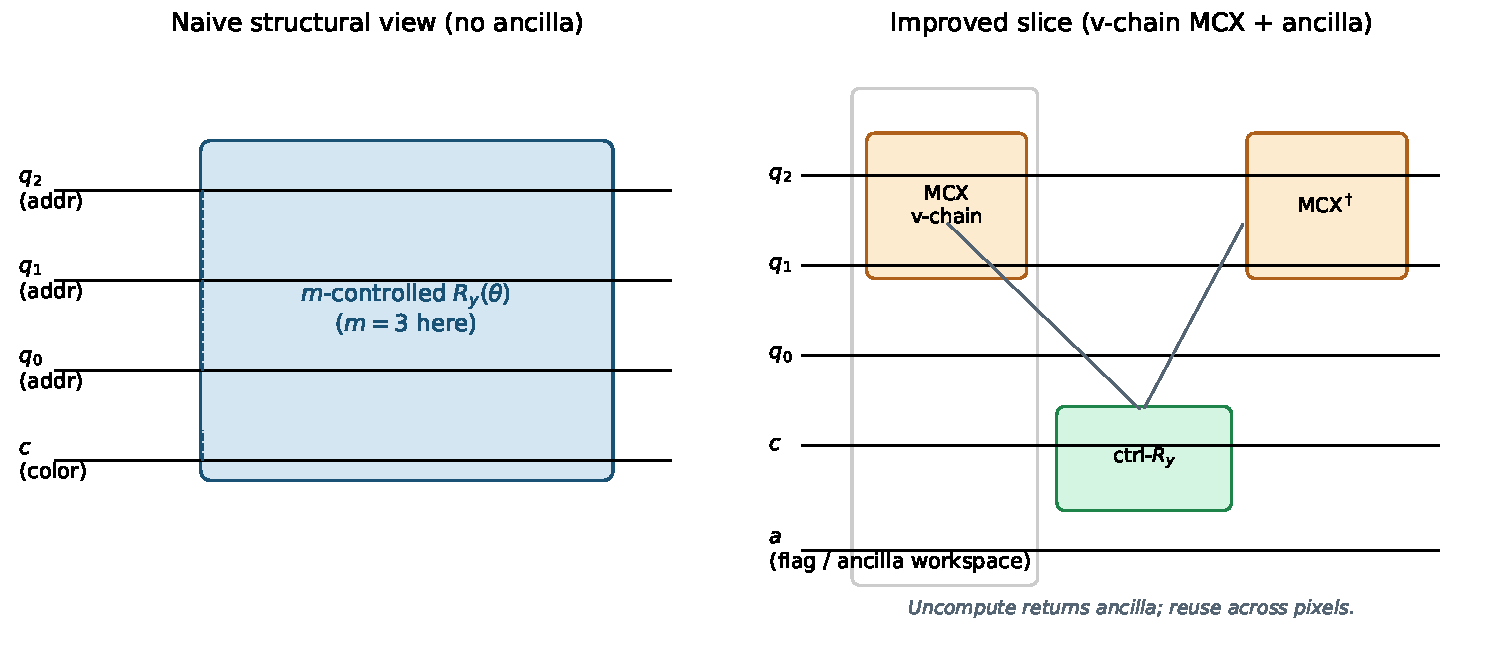
\includegraphics[width=\textwidth]{toy_naive_vs_vchain.pdf}
\caption{Toy $m{=}3$ address qubits and one color wire: naive ``all controls into one box'' versus v-chain ancilla workspace (repository figure \texttt{toy\_naive\_vs\_vchain}).}
\label{fig:toy-naive-vchain}
\end{figure}

\begin{figure}[htbp]
\centering
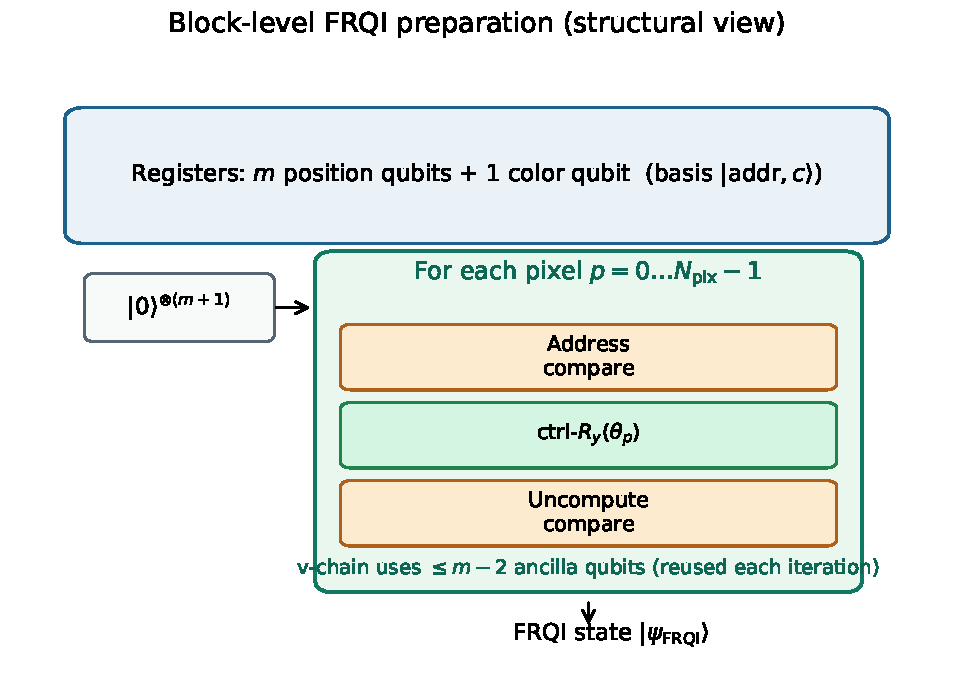
\includegraphics[width=0.92\textwidth]{block_frqi_prep.pdf}
\caption{Block-level view of the sequential FRQI preparation loop over pixels (registers, initialization, per-pixel compare--rotate--uncompute).}
\label{fig:block-frqi-prep}
\end{figure}

\FloatBarrier

\subsection{Transpiled excerpt (Qiskit \texttt{MCXGate} v-chain)}
\Cref{fig:stub-mcx} shows a minimal Qiskit circuit (saved from the repository stub helper) illustrating how a multi-controlled $X$ expands in v-chain mode before basis-gate transpilation, complementing the logical cartoons above.

\begin{figure}[H]
\centering
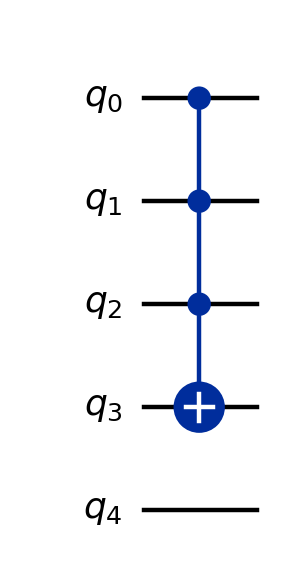
\includegraphics[width=0.55\textwidth]{stub_mcx_vchain.png}
\caption{Excerpt: \texttt{MCXGate} with \texttt{mode="v-chain"} on a few qubits (\texttt{outputs/stub\_mcx\_vchain.png}, from \texttt{scripts/qiskit\_stub\_draw.py}).}
\label{fig:stub-mcx}
\end{figure}

\FloatBarrier

\section{Decoding the simulated state into an image}
\label{sec:decode}
Decoding inverts the FRQI encoding: it reads the color-qubit amplitudes back out of the simulated state and rebuilds an ordinary grayscale raster $\hat{I}$. This is where the quantum stage hands off to the classical image-processing stage.

The simulator returns either a statevector (noiseless case) or a density matrix $\rho$ (noisy case). For every address $p$, the decoder reads the two populations at that address, $d_0\propto\cos^2\theta_p$ at index $2p$ and $d_1\propto\sin^2\theta_p$ at index $2p+1$, and recovers the angle from their ratio,
\begin{equation}
\hat{\theta}_p = \operatorname{atan2}\!\bigl(\sqrt{d_1},\,\sqrt{d_0}\bigr), \qquad \hat{I}[p] = \operatorname{round}\!\Bigl(255\cdot\frac{2\hat{\theta}_p}{\pi}\Bigr),
\label{eq:decode}
\end{equation}
which is just \Cref{eq:frqi-angle} solved for $I[p]$. Equivalently, the conditional probability of measuring color~$1$ at address $p$ is $P=d_1/(d_0+d_1)=\sin^2\theta_p$, so $\hat{\theta}_p=\arcsin\sqrt{P}$.

\paragraph{Worked round trip.}
Continuing the $I[p]=128$ example: encoding gave $\theta_p\approx 0.789$, so the conditional color-$1$ probability is $P=\sin^2(0.789)\approx 0.504$. Decoding inverts it as $\hat{\theta}_p=\arcsin\sqrt{0.504}\approx 0.789$ and $\hat{I}[p]=\operatorname{round}(255\cdot 2\cdot 0.789/\pi)=\operatorname{round}(128.1)=128$, recovering the original intensity exactly in the noiseless case.

Collecting all $N_{\mathrm{pix}}$ values on the $N\times N$ grid gives $\hat{I}$ in the \texttt{uint8} range. The statevector path reads $d_0,d_1$ from squared amplitudes (\srccode{src/frqi.py::reconstruct_image_from_statevector}); the noisy path reads them from the diagonal of $\rho$ after tracing out the irrelevant qubits, which is why it is called partial-trace decoding (\srccode{src/frqi.py::reconstruct_image_from_reduced_density_matrix}). From here on every quantity is computed on plain pixel arrays.

\section{QHED baseline and classical Sobel reference}
The quantum Hadamard edge detector (QHED) is the downstream operator that turns the reconstructed image into an edge map. It is held fixed throughout the thesis, so any change in scores can be attributed to FRQI preparation rather than to the detector. The pipeline below is implemented in \srccode{src/qhed.py::baseline_qhed_edge_map} (with the reference produced by \srccode{src/qhed.py::classical_sobel_edge_map}) as a sequence of array operations on the decoded raster $\hat{I}$~\cite{Yao2017QHED,QiskitTextbookQuantumEdgeDetection}.

\begin{enumerate}[label=\textbf{\arabic*.}, leftmargin=*]
  \item \textbf{Input.} Start from the decoded $N\times N$ image $\hat{I}$ of \Cref{sec:decode}.
  \item \textbf{Walsh--Hadamard transform.} Apply a fast Walsh--Hadamard transform (FWHT) along rows and then columns. The FWHT is a close cousin of the Fourier transform but uses only additions and subtractions: it repeatedly forms sums and differences of pairs of values, so it measures how strongly the image changes between neighbouring positions. Sharp changes (edges) produce large coefficients; flat regions produce small ones.
  \item \textbf{Magnitude spectrum.} Take the absolute value of the coefficients. This keeps the \emph{strength} of each change while dropping its sign, giving a contrast map in the transform domain.
  \item \textbf{Inverse transform.} Apply the inverse FWHT to bring the contrast map back to the spatial layout, so high values sit where the image varies strongly.
  \item \textbf{Sobel reference.} Independently, apply the classical $3\times 3$ Sobel magnitude filter (defined in \Cref{sec:classical-metrics}) to the original clean image. This is the reference edge map that QHED is scored against.
\end{enumerate}

Scoring compares two edge maps: QHED on the (possibly noisy) reconstruction, and Sobel on the clean reference (the scoring box of \Cref{fig:pipeline-flow}). Because QHED is a Walsh--Hadamard contrast detector and not a literal Sobel filter, the two maps differ in shape even with no noise. Edge SSIM is therefore below $1$ in the ideal case, so the thesis reports QHED-versus-Sobel SSIM as a \emph{relative} indicator across preparation modes rather than an absolute quality score.

\section{Noise model}
The noisy runs replace exact simulation with a depolarizing channel that models the gate errors of near-term hardware, so the experiments can ask how preparation quality survives noise. Noisy simulations use Qiskit Aer with the \texttt{density\_matrix} method. A single-qubit depolarizing probability $p_1$ and a two-qubit $p_2$ act on a density matrix $\rho$ as
\begin{equation}
\mathcal{E}_{\mathrm{1q}}(\rho) = (1-p_1)\rho + \frac{p_1}{3}\sum_{k\in\{X,Y,Z\}} P_k \rho P_k^\dagger ,
\end{equation}
and similarly for the two-qubit channel on each CX site (assembled by \srccode{src/noise_models.py::build_noise_model} and executed via \srccode{src/noise_models.py::run_density_matrix}). Thermal-relaxation and readout hooks exist for API compatibility, but unless a shot-based readout demo is enabled, readout noise does not alter the stored density matrix in the main noisy sweeps. \Cref{tab:noise-grid} lists the synthetic noise grid.

\begin{table}[htbp]
\centering
\caption{Synthetic noise grid used in the primary CSV bundle (each scale multiplies the baseline channel strengths).}
\label{tab:noise-grid}
\begin{tabular}{lrr}
\toprule
\texttt{noise\_scale} & $p_1$ (1q depolar) & $p_2$ (2q depolar) \\
\midrule
$0.0$ & $0$ & $0$ \\
$0.05$ & $0.0002$ & $0.001$ \\
$0.1$ & $0.0004$ & $0.002$ \\
$0.15$ & $0.0006$ & $0.003$ \\
$0.2$ & $0.0008$ & $0.004$ \\
\bottomrule
\end{tabular}
\end{table}

\section{Image and quantum metrics}
Let $\hat{I}$ be an $N\times N$ reconstruction and $I$ the ground truth. The metrics reuse the definitions in \Cref{sec:classical-metrics}: mean squared error is $\mathrm{MSE}=\frac{1}{N_{\mathrm{pix}}}\sum_p (\hat{I}[p]-I[p])^2$, and peak SNR is
\begin{equation}
\mathrm{PSNR} = 10\log_{10}\frac{255^2}{\mathrm{MSE}} \quad (\mathrm{dB}) .
\end{equation}
SSIM is computed with scikit-image on \texttt{uint8} arrays (windowed, channel-wise for grayscale). State fidelity
\begin{equation}
F(\rho,\sigma)=\bigl(\mathrm{Tr}\sqrt{\sqrt{\rho}\,\sigma\sqrt{\rho}}\bigr)^2
\end{equation}
compares the simulated noisy state (partial-traced to the data register) with the ideal FRQI statevector.

\paragraph{How to read these numbers.}
In plain terms: a higher PSNR (in decibels) means the reconstruction is closer to the original pixel by pixel, because it comes from a smaller MSE. SSIM closer to $1$ means local structure and contrast are preserved as a human eye would judge them, not just average brightness. Fidelity closer to $1$ means the noisy quantum state is close to the ideal FRQI state \emph{before} any image is decoded, so it measures damage at the quantum level. Edge SSIM applies the same structural-similarity idea to the two edge maps, so it reports how well the detected edges agree rather than how well the raw intensities match. Reporting all four together is deliberate: a preparation mode can improve one while leaving the others flat, and the thesis avoids hiding such mismatches behind a single headline number.

\section{Readout mitigation (shot-based slice)}
This slice corrects for measurement error rather than gate error: a calibration (confusion) matrix is estimated and inverted so that biased shot counts can be debiased. Separately from the depolarizing density-matrix runs, projective measurements on the color qubit are simulated with a synthetic confusion matrix $A$: outcome probabilities are estimated from finite shots (\srccode{src/noise_models.py::estimate_single_qubit_readout_matrix}), then a regularized inverse (\srccode{src/noise_models.py::invert_readout_matrix}) yields mitigated probabilities via \srccode{src/noise_models.py::mitigate_linear}~\cite{Mu2025GuidedImageFiltering}. Notation follows \texttt{thesis/design/readout\_mitigation.md}; the code entry point is \srccode{scripts/readout_mitigation_shot_sweep.py::main}, and the full pipeline is given in \Cref{sec:pipe-e5}.

\section{Statistical comparisons}
Because the sample sizes are small, the thesis uses paired non-parametric tests and treats every result as exploratory. For paired naive-versus-v-chain edge metrics, it reports exploratory Wilcoxon signed-rank tests on the differences $\Delta = \mathrm{vchain}-\mathrm{naive}$ over the eight $(\mathrm{image},\mathrm{noise\_scale})$ pairs with $\mathrm{noise\_scale}>0$ in the primary bundle. Readout mitigation pairs per-seed differences $\Delta_{\mathrm{seed}} = p_{1,\mathrm{mit}}-p_{1,\mathrm{raw}}$. These tests are \textbf{hypothesis-generating} only: multiplicity across metrics is not adjusted and sample sizes are small.

\paragraph{What the Wilcoxon signed-rank test is.}
The Wilcoxon signed-rank test is a paired, non-parametric test that asks whether the signed differences $\Delta$ within matched pairs are symmetrically centered on zero. It works on ranks rather than raw values: it sorts the pairs by the \emph{absolute} size of their difference, assigns ranks, and then sums those ranks separately for the positive and negative differences. If naive and v-chain were interchangeable, the two rank sums would be similar; a lopsided split (the test statistic reported as \texttt{stat.}) indicates that one mode tends to score higher. Because it uses only the order of the differences, it makes no normality assumption, which suits these metric deltas: $n$ is small and quantities such as edge SSIM are bounded and visibly non-Gaussian, so a paired $t$-test would be hard to justify. A small $p$-value means the observed imbalance would be unlikely under the no-difference hypothesis; it does \emph{not} measure the size or practical importance of the effect, and with several metrics tested at once a single small $p$ can arise by chance. This is why the thesis reads these $p$-values together with the median $\Delta$ and treats them as exploratory.

\paragraph{Inclusion protocol.}
A row enters the edge-metric pairing only if both \texttt{edge\_ssim\_naive} and \texttt{edge\_ssim\_vchain} are finite for the same tuple $(\mathrm{image},\mathrm{noise\_scale},\mathrm{topology},\mathrm{noise\_mode})$. At $16\times 16$, v-chain columns are often \texttt{NaN} because density-matrix simulation is skipped, so those cells are excluded automatically; this reduces power but avoids imputing synthetic values. The test is SciPy's two-sided Wilcoxon on paired differences, and exact $p$-values are available because $n{=}8$ is small.

\paragraph{Interpretation guardrails.}
Even if $p<0.05$ appears for a secondary metric such as fidelity, no claim of ``statistically significant superiority of v-chain for edge quality'' is made unless the edge-centric endpoints agree. Resource reductions and fidelity shifts can coexist with flat or negative edge SSIM, because QHED couples nonlinearly to reconstruction noise and the Sobel reference is not matched to QHED's spectral stage~\cite{Geng2022HybridNISQEdge}.

\section{Experiment pipelines}
\label{sec:pipelines}
The conceptual sections above describe each stage in isolation. This section ties them together by walking through every experiment end to end and naming the exact code path for each step, written as \srccode{file.py::function}. Each pipeline is presented twice: as a numbered step table that maps ``what happens'' to its routine and output, and as a compact flow diagram that reuses the box/arrow style of \Cref{fig:pipeline-flow}. \Cref{tab:pipe-overview} gives the bird's-eye view; the subsections expand one experiment each.

\begin{table}[H]
\centering\footnotesize
\caption{Overview of the experiment pipelines, their driver scripts, core routines, and primary artifacts.}
\label{tab:pipe-overview}
\begin{tabular}{@{}p{0.5cm}p{2.4cm}p{4.6cm}p{4.4cm}@{}}
\toprule
& Driver script & Core routine & Primary output \\
\midrule
E1 & \srccode{frqi_qhed_sobel.py} & \srccode{run_case} & \srccode{frqi_qhed_sobel_metrics.csv} \\
E2 & \srccode{frqi_structural_resources.py} & \srccode{main}/\srccode{_row} & \srccode{frqi_structural_metrics.csv} \\
E3 & \srccode{noisy_frqi_sweep.py} & \srccode{noisy_frqi_metrics_row} & \srccode{noisy_frqi_metrics.csv} \\
E4 & \srccode{noisy_recon_qhed_edge_metrics.py} & \srccode{main} & \srccode{noisy_recon_qhed_edges.csv} \\
E5 & \srccode{readout_mitigation_shot_sweep.py} & \srccode{main} & \srccode{readout_mitigation_shot_sweep.csv} \\
\bottomrule
\end{tabular}
\end{table}

\subsection{E1: Ideal FRQI + QHED baseline}
\label{sec:pipe-e1}
\emph{Purpose: establish the noiseless reference point, decoding quality, and \texttt{initialize}-based resource counts.}

\begin{table}[H]\centering\footnotesize
\caption{Ideal FRQI+QHED baseline pipeline (\srccode{scripts/frqi_qhed_sobel.py::run_case}).}
\label{tab:pipe-ideal}
\begin{tabular}{@{}p{0.5cm}p{3.9cm}p{5.6cm}p{2.4cm}@{}}
\toprule
\# & What happens & Code (\texttt{file::function}) & Output \\
\midrule
1 & Load \texttt{uint8} test image & \srccode{frqi_qhed_sobel.py::_load} & $N\times N$ array \\
2 & Build ideal FRQI statevector & \srccode{src/frqi.py::build_frqi_statevector} & $\ket{\psi}$ \\
3 & Decode statevector to raster & \srccode{src/frqi.py::reconstruct_image_from_statevector} & $\hat I$ \\
4 & QHED + Sobel edge maps & \srccode{src/qhed.py::baseline_qhed_edge_map}, \srccode{classical_sobel_edge_map} & edge maps \\
5 & Quality metrics & \srccode{src/metrics.py::psnr}, \srccode{ssim_uint8}, \srccode{ssim_like}, \srccode{src/frqi.py::l2_error} & CSV row \\
6 & Transpiled resources & \srccode{src/frqi.py::maybe_build_qiskit_circuit}, \srccode{src/resources.py::transpiled_circuit_stats} & qubits/CX/depth \\
\bottomrule
\end{tabular}
\end{table}

\begin{figure}[H]
\centering
\resizebox{\textwidth}{!}{%
\begin{tikzpicture}[
  font=\small,
  box/.style={rectangle, draw, rounded corners=2pt, align=center, inner sep=5pt, minimum width=2.2cm},
  arrow/.style={-{Stealth[length=2.2mm]}, thick},
]
\node[box, fill=blue!8] (load) {Load image\\\srccode{_load}};
\node[box, fill=blue!8, right=0.7cm of load] (sv) {FRQI SV\\\srccode{build_frqi_statevector}};
\node[box, fill=green!10, right=0.7cm of sv] (dec) {Decode\\\srccode{reconstruct_image_from_statevector}};
\node[box, fill=green!10, right=0.7cm of dec] (qhed) {QHED+Sobel\\\srccode{baseline_qhed_edge_map}};
\node[box, fill=orange!12, right=0.7cm of qhed] (score) {Metrics\\\srccode{psnr}, \srccode{ssim_uint8}};
\draw[arrow] (load) -- (sv);
\draw[arrow] (sv) -- (dec);
\draw[arrow] (dec) -- (qhed);
\draw[arrow] (qhed) -- (score);
\end{tikzpicture}%
}
\caption{E1 ideal baseline flow: a single clean image is encoded, decoded, edge-detected, and scored, with transpiled resources read off the \texttt{initialize} circuit.}
\label{fig:pipe-ideal}
\end{figure}

\subsection{E2: Structural resource scaling}
\label{sec:pipe-e2}
\emph{Purpose: compare naive versus v-chain CX and depth as the image grows, using transpiled circuit statistics.}

\begin{table}[H]\centering\footnotesize
\caption{Structural resource pipeline (\srccode{scripts/frqi_structural_resources.py::main}).}
\label{tab:pipe-structural}
\begin{tabular}{@{}p{0.5cm}p{3.9cm}p{5.6cm}p{2.4cm}@{}}
\toprule
\# & What happens & Code (\texttt{file::function}) & Output \\
\midrule
1 & Build v-chain prep circuit & \srccode{src/improved.py::build_frqi_prep_vchain} & circuit \\
2 & Build naive prep ($4\times4$ full) & \srccode{src/improved.py::build_frqi_prep_naive} & circuit \\
3 & Build naive slice ($8\times8$, $16\times16$) & \srccode{src/improved.py::build_single_address_ry_slice} & slice $\times N_{\mathrm{pix}}$ \\
4 & Transpile and count CX/depth & \srccode{src/resources.py::transpiled_circuit_stats} & per-mode stats \\
5 & Emit CSV rows & \srccode{frqi_structural_resources.py::_emit_csv}, \srccode{_row} & \srccode{frqi_structural_metrics.csv} \\
6 & Plot CX/depth vs size & \srccode{frqi_structural_resources.py::plot_structural_metrics_csv} & \srccode{fig_cx_vs_image_size.png}, \srccode{fig_depth_vs_image_size.png} \\
\bottomrule
\end{tabular}
\end{table}

\begin{figure}[H]
\centering
\resizebox{\textwidth}{!}{%
\begin{tikzpicture}[
  font=\small,
  box/.style={rectangle, draw, rounded corners=2pt, align=center, inner sep=5pt, minimum width=2.2cm},
  arrow/.style={-{Stealth[length=2.2mm]}, thick},
]
\node[box, fill=blue!8] (vc) {v-chain prep\\\srccode{build_frqi_prep_vchain}};
\node[box, fill=blue!8, below=0.45cm of vc] (nv) {naive prep / slice\\\srccode{build_frqi_prep_naive}};
\node[box, fill=green!10, right=1.0cm of vc] (tr) {Transpile + count\\\srccode{transpiled_circuit_stats}};
\node[box, fill=orange!12, right=1.0cm of tr] (csv) {CSV + plots\\\srccode{plot_structural_metrics_csv}};
\draw[arrow] (vc) -- (tr);
\draw[arrow] (nv) -| (tr);
\draw[arrow] (tr) -- (csv);
\end{tikzpicture}%
}
\caption{E2 structural resource flow: both synthesis modes are transpiled to \texttt{\{cx,rz,sx\}} and their CX/depth tabulated and plotted against image size.}
\label{fig:pipe-structural}
\end{figure}

\subsection{E3: Noisy FRQI sweep (density matrix)}
\label{sec:pipe-e3}
\emph{Purpose: measure how depolarizing noise degrades fidelity and reconstruction quality across the noise grid of \Cref{tab:noise-grid}.}

\begin{table}[H]\centering\footnotesize
\caption{Noisy FRQI density-matrix pipeline (\srccode{src/noise_models.py::noisy_frqi_metrics_row}, driven by \srccode{scripts/noisy_frqi_sweep.py::main}).}
\label{tab:pipe-noisy}
\begin{tabular}{@{}p{0.5cm}p{3.9cm}p{5.6cm}p{2.4cm}@{}}
\toprule
\# & What happens & Code (\texttt{file::function}) & Output \\
\midrule
1 & Build prep circuit (naive/v-chain) & \srccode{src/improved.py::build_frqi_prep_vchain}, \srccode{build_frqi_prep_naive} & circuit \\
2 & Assemble noise model & \srccode{src/noise_models.py::build_noise_model}, \srccode{src/nisq_mock.py::noise_model_from_backend} & noise model \\
3 & Run density-matrix simulation & \srccode{src/noise_models.py::run_density_matrix} & $\rho$ \\
4 & Reduce to data register & \srccode{src/noise_models.py::reduced_frqi_density_matrix} & $\rho_{\mathrm{data}}$ \\
5 & State fidelity vs ideal & \srccode{state_fidelity} vs \srccode{src/frqi.py::build_frqi_statevector} & $F$ \\
6 & Decode + image metrics & \srccode{src/frqi.py::reconstruct_image_from_reduced_density_matrix}, \srccode{psnr}, \srccode{ssim_uint8} & CSV row \\
\bottomrule
\end{tabular}
\end{table}

\begin{figure}[H]
\centering
\resizebox{\textwidth}{!}{%
\begin{tikzpicture}[
  font=\small,
  box/.style={rectangle, draw, rounded corners=2pt, align=center, inner sep=5pt, minimum width=2.2cm},
  arrow/.style={-{Stealth[length=2.2mm]}, thick},
]
\node[box, fill=blue!8] (prep) {Prep\\\srccode{build_frqi_prep_vchain}};
\node[box, fill=blue!8, right=0.65cm of prep] (nm) {Noise model\\\srccode{build_noise_model}};
\node[box, fill=green!10, right=0.65cm of nm] (dm) {DM run\\\srccode{run_density_matrix}};
\node[box, fill=green!10, right=0.65cm of dm] (red) {Reduce\\\srccode{reduced_frqi_density_matrix}};
\node[box, fill=orange!12, right=0.65cm of red] (sc) {Fidelity + decode\\\srccode{psnr}, \srccode{ssim_uint8}};
\draw[arrow] (prep) -- (nm);
\draw[arrow] (nm) -- (dm);
\draw[arrow] (dm) -- (red);
\draw[arrow] (red) -- (sc);
\end{tikzpicture}%
}
\caption{E3 noisy density-matrix flow: the prepared state runs through a depolarizing noise model, is reduced to the data register, and is scored by fidelity and decoded-image metrics.}
\label{fig:pipe-noisy}
\end{figure}

\subsection{E4: Noisy reconstruction to QHED edges}
\label{sec:pipe-e4}
\emph{Purpose: propagate the noisy reconstruction through QHED and score edge quality against the clean Sobel reference.}

\begin{table}[H]\centering\footnotesize
\caption{Noisy-reconstruction edge pipeline (\srccode{scripts/noisy_recon_qhed_edge_metrics.py::main}).}
\label{tab:pipe-noisy-edges}
\begin{tabular}{@{}p{0.5cm}p{3.9cm}p{5.6cm}p{2.4cm}@{}}
\toprule
\# & What happens & Code (\texttt{file::function}) & Output \\
\midrule
1 & Clean Sobel reference & \srccode{src/qhed.py::classical_sobel_edge_map} & ref edges \\
2 & Noisy recon (reuse E3 row) & \srccode{src/noise_models.py::noisy_frqi_metrics_row} (\srccode{return_recon=True}) & $\hat I_{\mathrm{noisy}}$ \\
3 & QHED on noisy recon & \srccode{src/qhed.py::baseline_qhed_edge_map} & noisy edges \\
4 & Edge metrics & \srccode{src/metrics.py::psnr}, \srccode{ssim_uint8} & CSV row \\
\bottomrule
\end{tabular}
\end{table}

\begin{figure}[H]
\centering
\resizebox{\textwidth}{!}{%
\begin{tikzpicture}[
  font=\small,
  box/.style={rectangle, draw, rounded corners=2pt, align=center, inner sep=5pt, minimum width=2.2cm},
  arrow/.style={-{Stealth[length=2.2mm]}, thick},
]
\node[box, fill=blue!8] (ref) {Sobel ref\\\srccode{classical_sobel_edge_map}};
\node[box, fill=blue!8, below=0.45cm of ref] (nz) {Noisy recon\\\srccode{noisy_frqi_metrics_row}};
\node[box, fill=green!10, right=1.0cm of nz] (qh) {QHED\\\srccode{baseline_qhed_edge_map}};
\node[box, fill=orange!12, right=1.0cm of qh] (sc) {Edge metrics\\\srccode{psnr}, \srccode{ssim_uint8}};
\draw[arrow] (nz) -- (qh);
\draw[arrow] (qh) -- (sc);
\draw[arrow] (ref) -| (sc);
\end{tikzpicture}%
}
\caption{E4 noisy-edge flow: QHED runs on the noisy reconstruction and the resulting edge map is compared with the clean classical Sobel reference.}
\label{fig:pipe-noisy-edges}
\end{figure}

\subsection{E5: Readout mitigation (shot-based slice)}
\label{sec:pipe-e5}
\emph{Purpose: demonstrate calibration-matrix inversion on a single-qubit readout slice with finite-shot statistics and bootstrap confidence intervals.}

\begin{table}[H]\centering\footnotesize
\caption{Readout mitigation pipeline (\srccode{scripts/readout_mitigation_shot_sweep.py::main}).}
\label{tab:pipe-readout}
\begin{tabular}{@{}p{0.5cm}p{3.9cm}p{5.6cm}p{2.4cm}@{}}
\toprule
\# & What happens & Code (\texttt{file::function}) & Output \\
\midrule
1 & Build single-address $R_y$ slice & \srccode{src/improved.py::build_single_address_ry_slice} & circuit \\
2 & Readout noise model & \srccode{src/noise_models.py::build_noise_model} & noise model \\
3 & Estimate confusion matrix $A$ & \srccode{src/noise_models.py::estimate_single_qubit_readout_matrix} & $A$ \\
4 & Invert calibration matrix & \srccode{src/noise_models.py::invert_readout_matrix} & $A^{-1}$ \\
5 & Transpile + run shots & \srccode{src/noise_models.py::transpile_for_aer_noise}, \srccode{run_shots_counts} & counts \\
6 & Counts $\to$ probs $\to$ mitigate & \srccode{src/noise_models.py::counts_to_prob_vector}, \srccode{mitigate_linear} & CSV row + CI \\
\bottomrule
\end{tabular}
\end{table}

\begin{figure}[H]
\centering
\resizebox{\textwidth}{!}{%
\begin{tikzpicture}[
  font=\small,
  box/.style={rectangle, draw, rounded corners=2pt, align=center, inner sep=5pt, minimum width=2.2cm},
  arrow/.style={-{Stealth[length=2.2mm]}, thick},
]
\node[box, fill=blue!8] (sl) {$R_y$ slice\\\srccode{build_single_address_ry_slice}};
\node[box, fill=blue!8, right=0.6cm of sl] (cal) {Calibrate $A$\\\srccode{estimate_single_qubit_readout_matrix}};
\node[box, fill=green!10, right=0.6cm of cal] (inv) {Invert\\\srccode{invert_readout_matrix}};
\node[box, fill=green!10, right=0.6cm of inv] (sh) {Run shots\\\srccode{run_shots_counts}};
\node[box, fill=orange!12, right=0.6cm of sh] (mit) {Mitigate\\\srccode{mitigate_linear}};
\draw[arrow] (sl) -- (cal);
\draw[arrow] (cal) -- (inv);
\draw[arrow] (inv) -- (sh);
\draw[arrow] (sh) -- (mit);
\end{tikzpicture}%
}
\caption{E5 readout-mitigation flow: a calibration matrix is estimated and inverted, then applied to finite-shot probabilities to recover mitigated estimates with bootstrap confidence intervals.}
\label{fig:pipe-readout}
\end{figure}

\subsection{E6: Results ingestion and table emission}
\label{sec:pipe-e6}
\emph{Purpose: validate the frozen CSVs and turn them into the thesis tables and figures.}

\begin{table}[H]\centering\footnotesize
\caption{Results-ingestion pipeline (\srccode{scripts/build_results_tables.py::main}/\srccode{ingest}).}
\label{tab:pipe-ingest}
\begin{tabular}{@{}p{0.5cm}p{3.9cm}p{5.6cm}p{2.4cm}@{}}
\toprule
\# & What happens & Code (\texttt{file::function}) & Output \\
\midrule
1 & Validate CSV columns & \srccode{build_results_tables.py::_validate_columns} & checked frames \\
2 & Build summary tables & \srccode{table_encoding_baseline}, \srccode{table_structural}, \srccode{pivot_noisy_edges}, \srccode{readout_summary} & data frames \\
3 & Paired statistics & \srccode{paired_naive_vchain_stats} & test results \\
4 & Emit \LaTeX{} + figures & \srccode{_write_bachelors_tex_fragment}, \srccode{emit_figures} & thesis tables/figures \\
\bottomrule
\end{tabular}
\end{table}

\section{Experimental setup}

\subsection{Simulator-only scope}
\textbf{All evidence is simulator-only.} No IBM Quantum hardware shots are included, due to lack of hardware access; results use Qiskit Aer backends and synthetic noise grids.

\subsection{Data and software}
Datasets live under \texttt{data/test\_images/} as \texttt{test\_4x4.npy}, \texttt{test\_8x8.npy}, and \texttt{test\_16x16.npy}. The Python environment is pinned in \texttt{requirements.txt} (Qiskit~1.x, Qiskit Aer, NumPy, SciPy, pandas, Matplotlib, scikit-image). The individual experiments and their end-to-end code paths are detailed in \Cref{sec:pipelines}; \Cref{tab:pipe-overview} maps each one to its driver script and primary artifact.

\subsection{Repository layout}
\Cref{fig:repo-tree} shows the high-level layout of the repository so the modules and scripts referenced throughout this chapter can be placed in context. The core \texttt{src/} package holds the quantum and image-processing routines, \texttt{scripts/} contains the reproducible experiment and build drivers, and \texttt{outputs/} stores the frozen artifacts the thesis ingests. The detailed mapping from each concern to its module and driver script is given in \Cref{tab:repo-map} (\Cref{sec:repo-map}).

\begin{figure}[H]
\centering
\begin{lstlisting}[language={}, basicstyle=\ttfamily\scriptsize, frame=single, breaklines=false, numbers=none, xleftmargin=0pt, framexleftmargin=4pt, columns=fixed]
qip-frqi-qhed.../            # repository root
|-- src/                     # core package: circuits, metrics, noise
|   |-- frqi.py              # FRQI angle encoding + partial-trace decode
|   |-- improved.py          # structural MCXGate modes (naive vs v-chain)
|   |-- qhed.py              # QHED + classical Sobel reference
|   |-- metrics.py           # PSNR, SSIM, state fidelity
|   |-- noise_models.py      # depolarizing density-matrix channels
|   |-- nisq_mock.py         # mock NISQ backend / noise-from-backend
|   |-- resources.py         # transpiled depth / CX accounting
|   +-- experiment_manifest.py     # provenance manifest writer
|-- scripts/                 # reproducible experiment + build drivers
|   |-- frqi_qhed_sobel.py            # ideal FRQI+QHED baseline + figures
|   |-- frqi_structural_resources.py  # structural CX/depth CSVs + plots
|   |-- noisy_frqi_sweep.py           # depolarizing DM noise sweep
|   |-- noisy_recon_qhed_edge_metrics.py  # noisy recon -> edge metrics
|   |-- readout_mitigation_shot_sweep.py  # calibration-matrix inversion
|   |-- build_results_tables.py       # validate CSVs -> thesis tables
|   +-- ...                            # diagram + build helpers
|-- tests/                   # pytest unit + monotonicity sweep tests
|-- data/
|   |-- test_images/         # test_4x4 / 8x8 / 16x16 .npy
|   +-- experiment_presets/  # weak / medium / strong noise YAMLs
|-- outputs/                 # frozen CSVs, JSON manifests, PNG figures
|-- thesis/                  # LaTeX sources, design notes, generated tables
|   |-- masters_en/          # this thesis document
|   +-- design/              # design notes + figure sources
|-- slides/                  # Beamer defence slides
|-- requirements.txt         # pinned Qiskit/Aer environment
|-- pytest.ini
|-- README.md
+-- LICENSE
\end{lstlisting}
\caption{High-level repository layout (curated): top-level directories with the key \texttt{src/} modules and \texttt{scripts/} drivers. The full module-to-script mapping is in \Cref{tab:repo-map}.}
\label{fig:repo-tree}
\end{figure}

\subsection{Transpilation settings}
Structural resource circuits are transpiled to basis gates \texttt{\{cx,rz,sx\}} at optimization level~3 with an unconstrained coupling map (resource study). The \textbf{frozen noisy bundles} referenced in \texttt{thesis/results\_configuration.md} instead pin \texttt{transpile\_optimization\_level=0} together with Qiskit~1.3.3 / Aer~0.16.4 and seed~42; this isolates the noise sweeps from aggressive rewrite passes that could blur naive--v-chain comparisons. CSV columns from different optimization levels should not be mixed without re-running both tracks at a common setting.

\subsection{Reproducible commands}
Each command corresponds to a pipeline in \Cref{sec:pipelines}: E1~(\Cref{tab:pipe-ideal}), E2~(\Cref{tab:pipe-structural}), E3~(\Cref{tab:pipe-noisy}), E4~(\Cref{tab:pipe-noisy-edges}), E5~(\Cref{tab:pipe-readout}), and E6~(\Cref{tab:pipe-ingest}).
\begin{lstlisting}[language={}, basicstyle=\ttfamily\footnotesize, frame=single, breaklines=true]
# E1: Ideal FRQI + QHED figures and encoding CSV
python scripts/frqi_qhed_sobel.py

# E2: Structural resources (CSV + CX/depth plots)
python scripts/frqi_structural_resources.py

# E3: Noisy FRQI sweep (16x16 v-chain optional via --allow-heavy-dm)
python scripts/noisy_frqi_sweep.py

# E4: Noisy reconstruction -> QHED edge metrics (paired naive vs v-chain)
python scripts/noisy_recon_qhed_edge_metrics.py

# E5: Readout mitigation multi-seed demo
python scripts/readout_mitigation_shot_sweep.py

# E6: Regenerate thesis ingestion tables (requires PNGs if --require-figures)
python scripts/build_results_tables.py --require-figures
\end{lstlisting}

\subsection{Provenance}
Noisy and readout experiments are summarized in \texttt{thesis/results\_configuration.md}; the JSON manifests in \texttt{outputs/experiment\_manifest\_*.json} record the Qiskit version, the random seed, and Git commit hashes when available. Density-matrix simulation cost scales as $O(4^{n_q})$ in the worst case~\cite{NielsenChuang2010}, so $16\times 16$ v-chain rows may be absent unless heavy-memory flags are enabled, and \Cref{ch:results} flags missing cells explicitly.
